%\documentclass[aspectratio=169]{beamer} %para apresentações em widescreen
\documentclass[10pt]{beamer} %para apresentação normal
\logo{\includegraphics[height=1cm]{Imagens/logon.jpg}\vspace{220pt}}
\newcommand{\nologo}{\setbeamertemplate{logo}{}} % command to set the logo to nothing
\usetheme{default}
\usefonttheme{serif}
\usecolortheme{default}
%%%%%%%%%%%%%%%%%%%%PACOTES EXTRAS%%%%%%%%%%%%%%%%%%%
\usepackage[utf8]{inputenc}
\usepackage[T1]{fontenc}
\usepackage[portuguese, english]{babel}
\usepackage[round]{natbib}
\usepackage{hyperref} 
\usepackage{smartdiagram}
\usepackage{graphicx} % Required for including images
\usepackage{graphics}
\usepackage{subfigure}
\graphicspath{{Imagens/}} % Location of the graphics files
\usepackage{booktabs} % Top and bottom rules for table
\usepackage[font=small,labelfont=bf]{caption} % Required for specifying captions to tables and figures
\usepackage{amsfonts, amsmath, amsthm, amssymb} % For math fonts, symbols and environments
\usepackage{wrapfig} % Allows wrapping text around tables and figures
\usepackage{ucs}
\usepackage{amsmath}
\usepackage{amsfonts}
\usepackage{amssymb}
\usepackage{amsthm}
\usepackage{times}
%\usepackage{movie15}%pacote para acrescentar vídeos
%\usepackage{multimedia}
%\usepackage{media9}%pacote de vídeos em formato mp4
%\usepackage{flashmovie}%outro pacote para inserir vídeos
%\usepackage{graphicx} %The mode "LaTeX => PDF" allows the following formats: .jpg  .png  .pdf  .mps
%\graphicspath{{/Imagens}} %Where the figures folder is located
%\usepackage{media9}
%\addmediapath{/Imagens}
\usepackage{makeidx}
\usepackage{lipsum} % Required to insert dummy text. To be removed otherwise
\usepackage{epstopdf}%adiciona imagens em formato eps no pdf.
\usepackage{subfigure}%cria ambientes de multifiguras
\usepackage{float}%coloca as figuras exatamente aonde você quer
\usepackage{lipsum} % Required to insert dummy text. To be removed otherwise
%\usepackage{multicol, blindtext}%cria figura na página inteira
\hypersetup{colorlinks,breaklinks=true,urlcolor=color2,citecolor=color1,linkcolor=color1,bookmarksopen=false,pdftitle={Title},pdfauthor={Author}}%Comando adaptado para o texmaker do ubuntu 12.4 LTS
\definecolor{color1}{RGB}{0,0,90} % Color of the article title and sections
\definecolor{color2}{RGB}{0,20,20} % Color of the boxes behind the abstract and headings
\usepackage{verbatim}

%%%%%%%%%%%%%%%%%%%%%%%%%%%%%%%%%%%%%%%%%%%%%%%%%%%%%%%%%%%%%%%%%%%%%%%%%%%%%%%
%------------------------------FINAL DO PREÂMBULO------------------------------
%%%%%%%%%%%%%%%%%%%%%%%%%%%%%%%%%%%%%%%%%%%%%%%%%%%%%%%%%%%%%%%%%%%%%%%%%%%%%%%


\author[Carreira,V.R.]{Autor: Victor Carreira \\ Professor: Leandro Di Bartolo}
\title{Modelagem Numérica de Ondas Sísmicas}
\subtitle{Seminário}
\institute{Pós-Graduação \\ Observatório Nacional}
\date{Setembro de 2017}
\subject{xxx}
%\setbeamertemplate{footline}[frame number]
%\setbeamercovered{transparent}
%\setbeamertemplate{navigation symbols}{}
% Tela cheia
\hypersetup{pdfpagemode=FullScreen}

\usepackage{ragged2e}
\justifying



%----------------------------------------------------------------------------------------
%	SEPARAÇÃO DE SÍLABAS (Exemplos)
%----------------------------------------------------------------------------------------

\hyphenation{co-o-pe-ra-ção} 
\hyphenation{a-com-pa-nha-do} 
\hyphenation{nor-ma-li-za-ção} 
\hyphenation{nor-ma-li-za-do}
%-------------------------------------------------------------------------------------------

\begin{document}

\bgroup
\makeatletter
\setbeamertemplate{footline}
\makeatother
{\nologo
\begin{frame}
%\titlepage
\begin{figure}
\centering
\includegraphics[scale=0.4]{Imagens/logonvertical.jpg} 
\end{figure}
\end{frame}
}
\textsc{}\maketitle
\egroup 
\addtobeamertemplate{navigation symbols}{}{\hskip6pt\raisebox{2pt}{\color{blue}\insertframenumber}}
\setcounter{framenumber}{0}
\AtBeginSection[]
{ \begin{frame}
\centering
\frametitle{Sumário}

\tableofcontents[currentsection,currentsubsection]% apresenta o sumário antes de cada seção

\end{frame} }


%%%%%%%%%%%%%%%%%%%%%%%%%%%%%%%%%%%%%%%%%%%%%%%%%%%%%%%%%%%%%%%%%%%%%%%%%%%%
%-----------------------------INTRODUÇÃO---------------------------------
%%%%%%%%%%%%%%%%%%%%%%%%%%%%%%%%%%%%%%%%%%%%%%%%%%%%%%%%%%%%%%%%%%%%%%%%%%%%
\section{Introdução}

\begin{frame}
	\frametitle{Introdução}
	\transboxin%efeito de transição	
	\begin{block}{Esta apresentação versará sobre:}
		\begin{itemize}
			\pause
			\item Modelagem numérica utilizando o método das diferenças finitas de $2^{a}$ ordem;
			\pause %adiciona pausas entre os itens
			\item Onda acústica ;
			\pause
			\item Meio isotrópico e homogêneo;
			\pause
			\item Malha simples e bi-dimensional;
			\pause
			\item Condições de contorno não-reflexivas (One-way $1$D e CERJAN para uma borda);
			\pause
			\item Controle de versão.
			
			
		\end{itemize}	
	\end{block}
	
\end{frame}






	
	
	
%\begin{frame}
%\frametitle{Introdução}
%\framesubtitle{RNA}
%
%\begin{block}{O que define um neurônio artificial?}
%\pause
%Segundo o trabalho pioneiro de \citet{McCulloch1943} um neurônio artificial pode ser descrito de acordo com a Eq. \ref{Eq.neuronio-McCulloch}.
%\end{block}
%
%\begin{eqnarray}
%y=\theta \left( \sum^{n}_{j=1} w_{j} x_{j} -u \right)
%\label{Eq.neuronio-McCulloch}
%\end{eqnarray}
%\begin{itemize}
%\pause
%\item $\theta$ é o passo dado na posição $0$;
%\pause
%\item $w_{j}$ é chamada sinapse-peso associado a um $j_{esimo}$ \textit{input};
%\pause
%\item $u$ é função de ativação ou limite;
%\pause 
%\end{itemize}
%\end{frame}


%%%%%%%%%%%%%%%%%%%%%%%%%%%%%%%%%%%%%%%%%%%%%%%%%%%%%%%%%%%%%%%%%%%%%%%%%%%%
%--------------------------CONTROLE DE VERSÃO-------------------------------
%%%%%%%%%%%%%%%%%%%%%%%%%%%%%%%%%%%%%%%%%%%%%%%%%%%%%%%%%%%%%%%%%%%%%%%%%%%%
\section{Controle de Versão}

\begin{frame}
\frametitle{Controle de Versão}
\transboxin

\begin{block}{O que é isso?}
\begin{figure}[H]
\centering
\includegraphics[scale=0.3]{Imagens/pensador.png}
\end{figure}
\end{block}

\end{frame}

\begin{frame}
\frametitle{Controle de Versão}
\transboxin

\begin{block}{Imagine que...}
\begin{figure}[H]
\centering
\includegraphics[scale=0.3]{Imagens/versao_caso1.png}
\end{figure}

\end{block}
\end{frame}

\begin{frame}
\frametitle{Controle de Versão}


\begin{block}{Imagine que...}
\begin{figure}[H]
\centering
\includegraphics[scale=0.3]{Imagens/versao_caso2.png}
\end{figure}

\end{block}
\end{frame}

\begin{frame}
\frametitle{Controle de Versão}


\begin{block}{Imagine que...}
\begin{figure}[H]
\centering
\includegraphics[scale=0.3]{Imagens/versao_caso3.png}
\end{figure}

\end{block}
\end{frame}

\begin{frame}
\frametitle{Controle de Versão}


\begin{block}{Imagine que...}
\begin{figure}[H]
\centering
\includegraphics[scale=0.3]{Imagens/versao_caso4.png}
\end{figure}

\end{block}
\end{frame}

\begin{frame}
\frametitle{Controle de Versão}


\begin{block}{Imagine que...}
\begin{figure}[H]
\centering
\includegraphics[scale=0.3]{Imagens/versao_caso5.png}
\end{figure}

\end{block}
\end{frame}

\begin{frame}
\frametitle{Controle de Versão}


\begin{block}{Imagine que...}
\begin{figure}[H]
\centering
\includegraphics[scale=0.3]{Imagens/versao_caso6.png}
\end{figure}

\end{block}
\end{frame}

\begin{frame}
\frametitle{Controle de Versão}

\begin{block}{Imagine que...}
\begin{figure}[H]
\centering
\includegraphics[scale=0.3]{Imagens/versao_caso7.png}
\end{figure}

\end{block}
\end{frame}


\begin{frame}
	\frametitle{Controle de Versão}
	\begin{block}{É um sistema gerenciador de diferentes versões no desenvolvimento de um documento.}
	\end{block}
	
\end{frame}


\begin{frame}
	\frametitle{Controle de Versão}
	
	
\begin{block}{Existem vários sistemas de gerenciamento de versões}
		
\begin{figure}[h]

\center
\subfigure[CVS][CVS]{\includegraphics[width=2.5cm]{Imagens/CVS.png}}
\qquad
\subfigure[ref2][Bazaar]{\includegraphics[width=2.5cm]{Imagens/Bazaar.png}}
\qquad
\subfigure[ref2][Libre Source]{\includegraphics[width=2.5cm]{Imagens/libresource.png}}
\qquad
\subfigure[ref2][Subversion]{\includegraphics[width=2.5cm]{Imagens/Subversion.png}}
\qquad
\subfigure[ref2][Mercurial]{\includegraphics[width=2.5cm]{Imagens/Mercurial.png}}
\qquad
\subfigure[ref2][GitHub]{\includegraphics[width=2.5cm]{Imagens/Github.png}}
\caption{Os seis principais sistemas de controle de versão}

\end{figure}
	
\end{block}
	
\end{frame}

\begin{frame}
	\frametitle{Controle de Versão}
	
	
\begin{block}{Existem vários sistemas de gerenciamento de versões}
		
\begin{figure}[h]

\center
\subfigure[CVS][CVS]{\includegraphics[width=2.5cm]{Imagens/CVS.png}}
\qquad
\subfigure[ref2][Bazaar]{\includegraphics[width=2.5cm]{Imagens/Bazaar.png}}
\qquad
\subfigure[ref2][Libre Source]{\includegraphics[width=2.5cm]{Imagens/libresource.png}}
\qquad
\subfigure[ref2][Subversion]{\includegraphics[width=2.5cm]{Imagens/Subversion.png}}
\qquad
\subfigure[ref2][Mercurial]{\includegraphics[width=2.5cm]{Imagens/Mercurial.png}}
\qquad
\subfigure[ref2][GitHub]{\includegraphics[width=2.5cm]{Imagens/Githubbola.png}}
\caption{Os seis principais sistemas de controle de versão}

\end{figure}
	
\end{block}
	
\end{frame}




%%%%%%%%%%%%%%%%%%%%%%%%%%%%%%%%%%%%%%%%%%%%%%%%%%%%%%%%%%%%%%%%%%%%%%%%%%%%
%-------------------UTILIZAÇÃO DO GITHUB EM MNUM2017----------------
%%%%%%%%%%%%%%%%%%%%%%%%%%%%%%%%%%%%%%%%%%%%%%%%%%%%%%%%%%%%%%%%%%%%%%%%%%%%
\section{O GitHub no programa de modelagem}

\begin{frame}
\frametitle{O GitHub no programa de modelagem}

\begin{block}{Criando um login e senha}
\begin{figure}[H]
\centering
\includegraphics[scale=0.15]{Imagens/Github.png}
\end{figure}

\end{block}
\end{frame}

\begin{frame}
\frametitle{O GitHub no programa de modelagem}

\begin{block}{}
\begin{figure}[H]
\centering
\includegraphics[scale=0.2]{Imagens/paginainicial.png}
\end{figure}

\end{block}
\end{frame}

\begin{frame}
\frametitle{O GitHub no programa de modelagem}

\begin{block}{}
\begin{figure}[H]
\centering
\includegraphics[scale=0.2]{Imagens/paginainicial_e.png}
\end{figure}

\end{block}
\end{frame}

\begin{frame}
\frametitle{O GitHub no programa de modelagem}

\begin{block}{}
\begin{figure}[H]
\centering
\includegraphics[scale=0.2]{Imagens/novorepositorio.png}
\end{figure}

\end{block}
\end{frame}

\begin{frame}
\frametitle{O GitHub no programa de modelagem}

\begin{block}{}
\begin{figure}[H]
\centering
\includegraphics[scale=0.2]{Imagens/novorepositorio_e.png}
\end{figure}

\end{block}
\end{frame}


\begin{frame}
\frametitle{O GitHub no programa de modelagem}

\begin{block}{}
\begin{figure}[H]
\centering
\includegraphics[scale=0.2]{Imagens/comandosgerais.png}
\end{figure}

\end{block}
\end{frame}

\begin{frame}
\frametitle{O GitHub no programa de modelagem}

\begin{block}{}
\begin{figure}[H]
\centering
\includegraphics[scale=0.3]{Imagens/navegando.png}
\end{figure}

\end{block}
\end{frame}

\begin{frame}
\frametitle{O GitHub no programa de modelagem}

\begin{block}{}
\begin{figure}[H]
\centering
\includegraphics[scale=0.3]{Imagens/navegando_e.png}
\end{figure}

\end{block}
\end{frame}

\begin{frame}
\frametitle{O GitHub no programa de modelagem}

\begin{block}{}
\begin{figure}[H]
\centering
\includegraphics[scale=0.3]{Imagens/trab03.png}
\end{figure}

\end{block}
\end{frame}


\begin{frame}
\frametitle{O GitHub no programa de modelagem}

\begin{block}{}
\begin{figure}[H]
\centering
\includegraphics[scale=0.3]{Imagens/trab03_e.png}
\end{figure}

\end{block}
\end{frame}

\begin{frame}
\frametitle{O GitHub no programa de modelagem}

\begin{block}{}
\begin{figure}[H]
\centering
\includegraphics[scale=0.3]{Imagens/programa.png}
\end{figure}

\end{block}
\end{frame}

\begin{frame}
\frametitle{O GitHub no programa de modelagem}

\begin{block}{}
\begin{figure}[H]
\centering
\includegraphics[scale=0.3]{Imagens/programa_e.png}
\end{figure}

\end{block}
\end{frame}

\begin{frame}
\frametitle{O GitHub no programa de modelagem}

\begin{block}{}
\begin{figure}[H]
\centering
\includegraphics[scale=0.3]{Imagens/hist.png}
\end{figure}

\end{block}
\end{frame}

\begin{frame}
\frametitle{O GitHub no programa de modelagem}

\begin{block}{}
\begin{figure}[H]
\centering
\includegraphics[scale=0.3]{Imagens/hist_e.png}
\end{figure}

\end{block}
\end{frame}

\begin{frame}
\frametitle{O GitHub no programa de modelagem}

\begin{block}{}
\begin{figure}[H]
\centering
\includegraphics[scale=0.12]{Imagens/versoes.png}
\end{figure}

\end{block}
\end{frame}

\begin{frame}
\frametitle{O GitHub no programa de modelagem}

\begin{block}{}
\begin{figure}[H]
\centering
\includegraphics[scale=0.12]{Imagens/versoes_e.png}
\end{figure}

\end{block}
\end{frame}


%%%%%%%%%%%%%%%%%%%%%%%%%%%%%%%%%%%%%%%%%%%%%%%%%%%%%%%%%%%%%%%%%%%%%%%%%%%%
%----------------------------------------ONE-WAY----------------------------
%%%%%%%%%%%%%%%%%%%%%%%%%%%%%%%%%%%%%%%%%%%%%%%%%%%%%%%%%%%%%%%%%%%%%%%%%%%%
\section{One-way}


\begin{frame}
	\frametitle{Condição de contorno não-reflexiva}
	\framesubtitle{Esquema numérico}
	\begin{block}{}
		\begin{figure}[H]
			\centering
			\includegraphics[scale=0.5]{Imagens/meuesquema.png}
		\end{figure}
		
	\end{block}
\end{frame}

\begin{frame}
	\frametitle{Condição de contorno não-reflexiva}
	\framesubtitle{Parâmetros do modelo}
	\begin{block}{}
\begin{table}[h]
	\centering
	\begin{tabular}{r|lr}
		
		Par{\^a}metro & Valor de entrada \\ % Note a separação de col. e a quebra de linhas
		\hline                               % para uma linha horizontal
		 Comprimento na direção x         &  1500 \\
		Comprimento na direção z         &  1500 \\
		Tempo, t            & 2 \\
		Velocidade de onda p, c      & 1500 \\
	    Espacamento entre os pontos, h & 2           \\
		 Discretização temporal, dt&  $8,0^{-4}$ \\
		 Posição da fonte na posição horizontal, xfonte& 750 \\
		 Posição da fonte na posição vertical, zfonte& 750 \\
		 Amplitude da fonte& 10 \\
		 Frequência de corte, fcorte& 60 \\
		 Frequência de atenuação, fcer & $1,50^{-3}$\\
		 Número de cerjan, ncer& 100 \\
		 Critério de dispersão de segunda ordem, alfa2& 5\\
		 Critério de dispersão quarta ordem , alfa4&10\\
		Número de Iterações para levar de 1 para 2, beta&4\\
		Número de snapshots ,nsnap &  20 % não é preciso quebrar a última linha
		
	\end{tabular}
\end{table}
		
	\end{block}
\end{frame}


\begin{frame}
	\frametitle{Condição de contorno não-reflexiva}
	\framesubtitle{Fonte}
	\begin{block}{}
		\begin{equation}
			s(\vec{x},t)=A[2\pi(\pi f_{c} t_{d})^{2}-1]^{- \pi (\pi f_{c} t_{d})^{2}}% \delta (\vec{x}- \vec{x_{f}})
		\end{equation}
		\label{fonte}
	\end{block}
	
	\begin{block}{}
		\begin{figure}[H]
			\centering
			\includegraphics[scale=0.2]{Imagens/fonte.png}
		\end{figure}	
	\end{block}
\end{frame}	
	
\begin{frame}
		\frametitle{Condição de contorno não-reflexiva}
		\framesubtitle{Fonte}
		\begin{block}{}
			\begin{figure}[H]
				\centering
				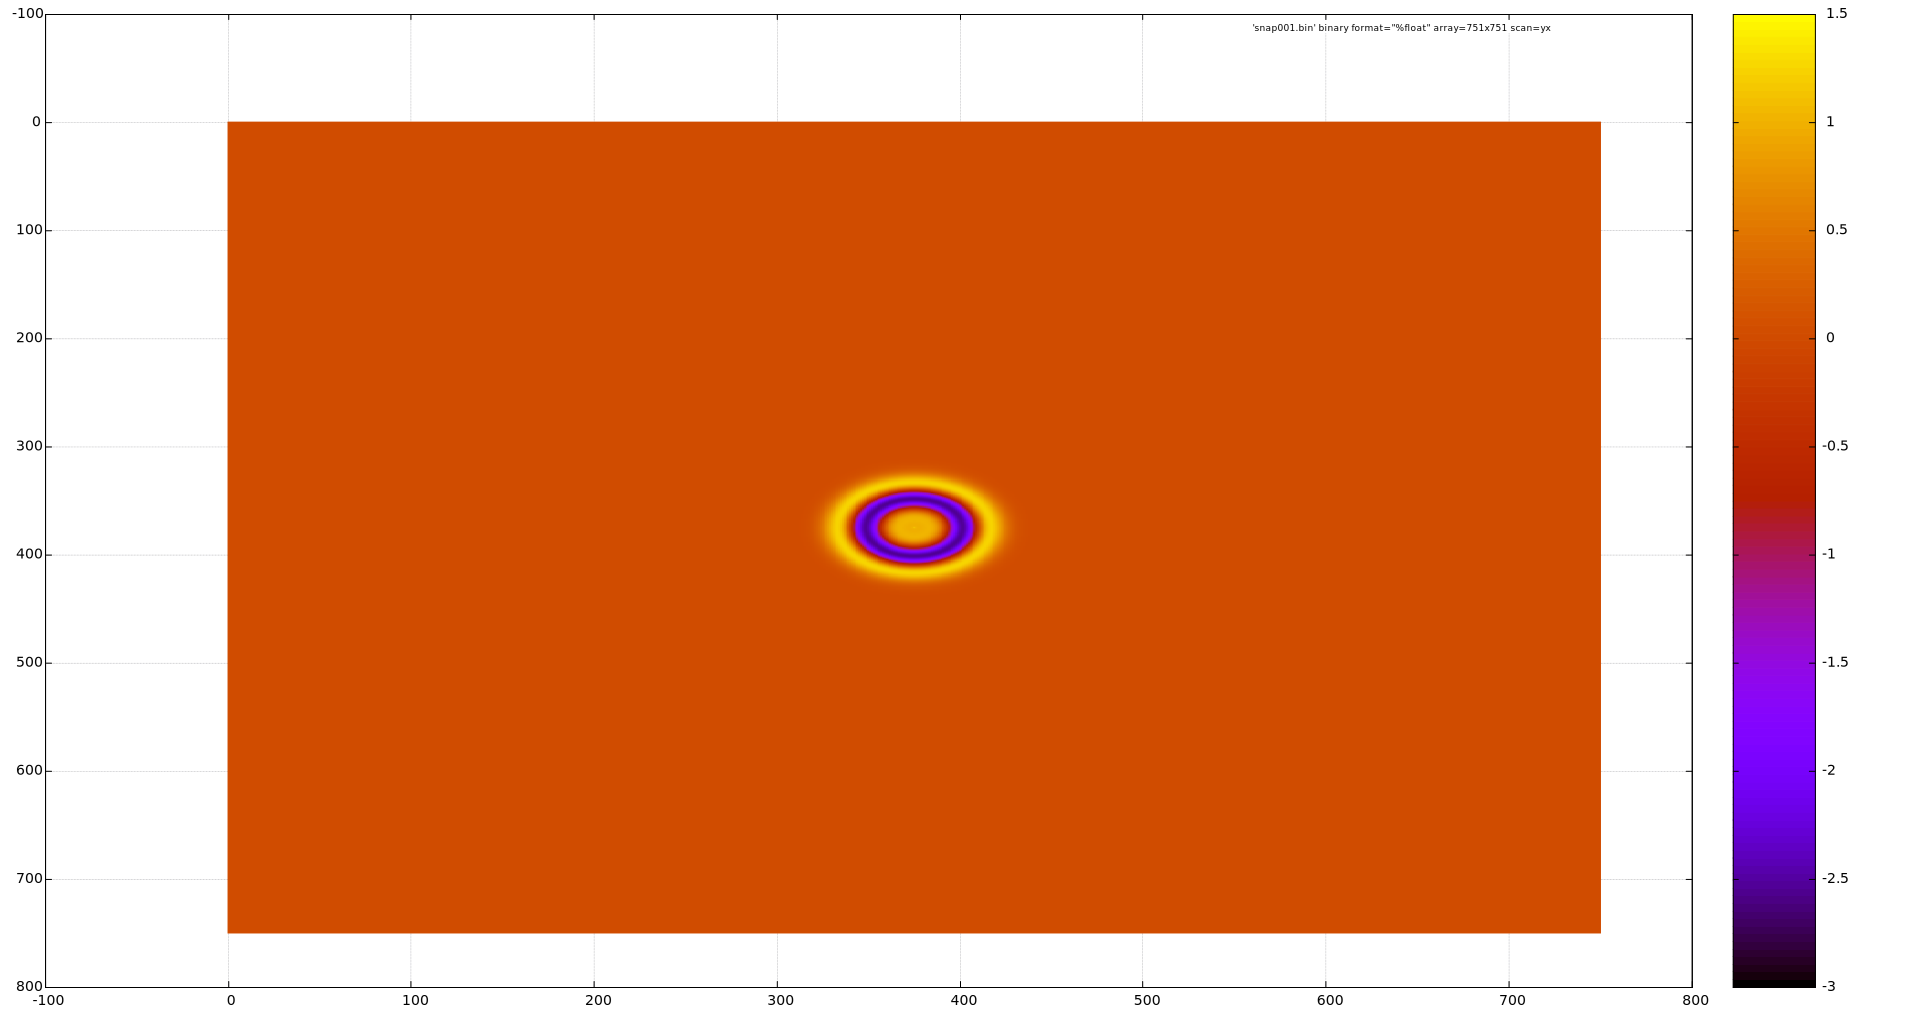
\includegraphics[scale=0.15]{Imagens/Snap001.png}
			\end{figure}
		\end{block}
\end{frame}
	
	


\begin{frame}
	\frametitle{Condição de contorno não-reflexiva}
	\framesubtitle{One-way $1$D}
	\begin{block}{Problemática}
	\begin{itemize}
	\item Presença de reflexões nas bordas do mesh numérico \citep{Cerjan1985};
	\pause
	\item Sobreposição desse efeitos maléficos sobre o sinal sísmico;
	\pause
	\end{itemize}
	\end{block}

\end{frame}

\begin{frame}
	\frametitle{Condição de contorno não-reflexiva}
	\framesubtitle{One-way $1$D}
	\begin{block}{Solução}
		\begin{itemize}
			\item Repor a equação da onda pela Eq Oneway;
			\pause 
			\item Impede que a energia se propague das bordas para dentro do mesh;
		\end{itemize}
	\end{block}
\end{frame}

%%%%%%%%%%%%%%%%%%%%%%%%%%%%%%%%%%%%%%%%%%%%%%%%%%%%%%%%%%%%%%%%%%%%%%%%%%%%
%---------------------------------------CERJAN------------------------------
%%%%%%%%%%%%%%%%%%%%%%%%%%%%%%%%%%%%%%%%%%%%%%%%%%%%%%%%%%%%%%%%%%%%%%%%%%%%
\section{Cerjan}

%%%%%%%%%%%%%%%%%%%%%%%%%%%%%%%%%%%%%%%%%%%%%%%%%%%%%%%%%%%%%%%%%%%%%%%%%%%%
%---------------------------------------RESULTADO---------------------------
%%%%%%%%%%%%%%%%%%%%%%%%%%%%%%%%%%%%%%%%%%%%%%%%%%%%%%%%%%%%%%%%%%%%%%%%%%%%
\section{Resultado final}


%  \begin{frame}
%    \begin{center}
%       \flashmovie[width=10cm]{Imagens/temporal.swf} 
%    \end{center}
%  \end{frame}


%\begin{frame}
%
%\centering % Para centralizarmos o vídeo
%\includemedia[
%label=nome_qualquer, % ! Importante para linkar o vídeo ao botão (ver abaixo)
%width=0.8\linewidth, height=0.5\linewidth, % Dimensões
%addresource=Imagens/temporal.swf, % ESTE É O SEU ARQUIVO DE VÍDEO (mesmo dir.)
%transparent, % Opções para que o player tenha transparência
%activate=pageopen, % Se você deseja que o vídeo esteja "carregado" ao abrir a página
%flashvars={
%source=Imagens/temporal.swf
%&loop=false % Se você quer que o vídeo repita automaticamente 
%&scaleMode=letterbox % Manter proporções (dimensionais) do vídeo
%}
%]{}{VPlayer.swf}
%\vspace{1cm} % Espaçamento entre vídeo e botão
%
%% Agora, você cria o botão para dar play/pause. Neste caso, o botão é apenas a letra "pi".
%
%\mediabutton[
%mediacommand=nome_qualquer:playPause,
%overface=\color{black}{{\strut $\pi$}},
%downface=\color{gray}{{\strut $\pi$}}
%]{{\strut $\pi$}}
%
%\end{frame}

%\begin{frame}
%\begin{figure}[h!]
%\centering    
%\movie[label=show3,width=1.0\textwidth,poster
%       ,autostart,showcontrols,loop] 
%  {\includegraphics[width=1.0\textwidth]{/snap1.png}}{temporal.mp4}
%  \caption{caption}
% \end{figure} 
%\end{frame}


%\begin{frame}
%\frametitle{Forward Kinematics}
%
%\begin{center}
%\includemedia[
%    activate=onclick,
%    width=0.75\textwidth
%]{\includegraphics{Imagens/snap1.png}}{Imagens/temporal.swf}
%\end{center}
%\end{frame}
%\begin{frame}
%
%\includemedia[width=0.6\linewidth,height=0.6\linewidth,activate=pageopen,
%passcontext,
%transparent,
%addresource=Imagens/temporal.mp4,
%flashvars={source=Imagens/temporal.mp4}
%]{\includegraphics[width=0.6\linewidth]{Imagens/snap1.png}}{Imagens/temporal.swf}
%
%\end{frame}
%%%%%%%%%%%%%%%%%%%%%%%%%%%%%%%%%%%%%%%%%%%%%%%%%%%%%%%%%%%%%%%%%%%%%%%%%%%%
%-----------------------------BIBLIORGRAFIA---------------------------------
%%%%%%%%%%%%%%%%%%%%%%%%%%%%%%%%%%%%%%%%%%%%%%%%%%%%%%%%%%%%%%%%%%%%%%%%%%%%

\section{Bibliografia}
	\begin{frame}[allowframebreaks]{Bibliografia}
	%\frametitle{Bibliografia}
	\beamertemplatetextbibitems
	\tiny
	\bibliographystyle{apalike}
	\bibliography{referencias.bib}
	\end{frame}

\makeatother
{\nologo
\begin{frame}
%\titlepage
\begin{figure}
\includegraphics[scale=0.25]{Imagens/logonvertical.jpg}
\end{figure}
\begin{center}
\begin{minipage}{0.77\textwidth}
\small
\begin{center}
Rua General José Cristino, 77 CEP 20921-400\\
Rua General Bruce, 586 CEP 20921-030\\
Bairro Imperial de São Cristóvão, Rio de Janeiro - RJ\\
PABX: 55 21 3504-9100\\
\url{www.on.br}
\end{center}
\end{minipage}
\end{center}
\end{frame}
}
\end{document}
